% arara: xelatex
\documentclass[12pt]{article}

\usepackage{tikz} % картинки в tikz
\usepackage{microtype} % свешивание пунктуации

\usepackage{array} % для столбцов фиксированной ширины

\usepackage{indentfirst} % отступ в первом параграфе

\usepackage{sectsty} % для центрирования названий частей
\allsectionsfont{\centering}

\usepackage{amsmath, amssymb, amsthm} % куча стандартных математических плюшек
\usepackage{amsfonts}
\usepackage{halloweenmath}

\usepackage{graphicx}

\usepackage{comment}

\usepackage[top=2cm, left=1.2cm, right=1.2cm, bottom=2cm]{geometry} % размер текста на странице

\usepackage{lastpage} % чтобы узнать номер последней страницы

\usepackage{enumitem} % дополнительные плюшки для списков
%  например \begin{enumerate}[resume] позволяет продолжить нумерацию в новом списке
% \usepackage{caption}

\usepackage{physics}

\usepackage{hyperref} % гиперссылки

\usepackage{multicol} % текст в несколько столбцов

\usepackage{url}

\usepackage{fancyhdr} % весёлые колонтитулы


\usepackage{todonotes} % для вставки в документ заметок о том, что осталось сделать
% \todo{Здесь надо коэффициенты исправить}
% \missingfigure{Здесь будет Последний день Помпеи}
% \listoftodos - печатает все поставленные \todo'шки


% более красивые таблицы
\usepackage{booktabs}
% заповеди из докупентации:
% 1. Не используйте вертикальные линни
% 2. Не используйте двойные линии
% 3. Единицы измерения - в шапку таблицы
% 4. Не сокращайте .1 вместо 0.1
% 5. Повторяющееся значение повторяйте, а не говорите "то же"



\usepackage{fontspec}
\usepackage{polyglossia}

\setmainlanguage{english}
\setotherlanguages{russian}

% download "Linux Libertine" fonts:
% http://www.linuxlibertine.org/index.php?id=91&L=1
\setmainfont{Linux Libertine O} % or Helvetica, Arial, Cambria
% why do we need \newfontfamily:
% http://tex.stackexchange.com/questions/91507/
\newfontfamily{\cyrillicfonttt}{Linux Libertine O}

\AddEnumerateCounter{\asbuk}{\russian@alph}{щ} % для списков с русскими буквами
% \setlist[enumerate, 2]{label=\asbuk*),ref=\asbuk*}


\let\P\relax
\DeclareMathOperator{\P}{\mathbb{P}}
\DeclareMathOperator{\plim}{plim}
\DeclareMathOperator{\E}{\mathbb{E}}
\newcommand{\cN}{\mathcal{N}}
\DeclareMathOperator{\Var}{\mathbb{V}ar}
\DeclareMathOperator{\Cov}{\mathbb{C}ov}
\DeclareMathOperator{\Corr}{\mathbb{C}orr}




\lhead{Олимпиада по теории вероятностей и статистике}
\rhead{2021-04-19, 18:10, R205}
\cfoot{\thepage} 

% версия для гостей ковидария (скрыты решения):
% \excludecomment{solution}
% версия для главврачей (открыты решения):
\newenvironment{solution}{}{}

\usepackage{epigraph}
\setlength\epigraphwidth{.6\textwidth}
\setlength\epigraphrule{0pt}


\title{Конкурс Псевдонаучных Исследовательских Плоскоземельных семинаров}
\date{}

% побег из ковидария или дистант в сумасшедшем доме

\begin{document}
	\maketitle

\section*{Правила}

Лженаучное руководство $\nu$-ШВЭ [Школы Волнового Экзорцизма] объявило конкурс ПИПСов [Псевдо\-на\-уч\-ных Исследовательских Плоскоземельных семинаров].
\begin{center}
    
\includegraphics[width=5cm]{zaryajeno.jpg}
\end{center}

Ваша задача организовать свой собственный ПИПС на четыре-пять человек. 
Ваш лженаучный ПИПС должен составить конкуренцию таким небезызвестным ПИПСам, как «Свидетели отрицательной вероят\-нос\-ти» [у них просто невероятные результаты],
«Депрессионный анализ» [у них весело], «Небинарные и квир-модели» [запись закрыта 5 декабря], «Приложение ложных импликаций к эконометрическому выводу» [не брезгуют ничем для достижения заказанных прогнозов].

Конкурс ПИПСов начинается 17 декабря в 17:12.
Регистрация ПИПСов на конкурс открыта до 11 декабря 23:59 по ссылке \url{https://forms.gle/LTZn2BcFu4KUAUNw9}.

Руководители и соруководители ПИПС в самых удачных костюмах получают дополнительные баллы. По итогам конкурса лучшие ПИПС получают грант Лженаучного фонда $\nu$-ШВЭ. На оценки по курсу теории вероятностей или статистики результаты конкурса не влияют. 

%\end{document}


\newpage

\section*{ЗБЧ: Задачи Белой Чакры}

\begin{enumerate}
    \item % задача 1
    $[+$5 в карму] Вероятность встретить аффинно очищенную молекулу антител к гамма интерферону в таблетке Анаферона составляет $10^{-8}$. Анаферон продают пачками по 20 таблеток.
    
    Сколько пачек лекарства нужно съесть, чтобы употребить молекулу данного вещества с вероятностью больше 0.5?

    % p(не употребить) < 0.5
    % (1 - 10^(-8))^(20*n) < 0.5
    % n >= 3465736
    
    \item  % задача 2
    $[+$5 в карму]  При полевых испытаниях Билл Гейтс выяснил что, когда нет никаких негативных факторов, его чипы работают с вероятностью $0.99$. При морозах вероятность работо\-спо\-собности чипа равна $0.95$. Если человек надевает шапочку из фольги, чип работает с веро\-ят\-нос\-тью $0.9$. Если человек надевает шапочку из фольги в мороз, то чип работает с вероятностью $0.8$. 

    В России морозы наступают с вероятностью $0.2$, а шапочку из фольги надевают с вероятностью $0.1$. 

    \begin{itemize}
    \item $[$+2 карму] Какова вероятность того, что чип отключится, если морозы и ношение шапочки из фольги не зависят друг от друга?
    
    \item $[$+3 карму] В каком диапазоне лежит вероятность того, что отключится чип, если морозы и ношение шапочки зависят друг от друга? 
    \end{itemize} 
    
    % % 0.2 * 0.1 * 0.2 + 0.2 * 0.9 * 0.05 + 0.8 * 0.1 * 0.1 + 0.8 * 0.9 * 0.99 = 0.7338
    
    \item  % задача 3
    $[+$5 в карму] В комнате общежития живут четыре студента $\nu$-ШВЭ. Инопланетяне в первую ночь похищают двух случайных студентов и проводят на них опыты, а потом возвращают обратно. На вторую ночь инопланетяне снова похищают двух случайных студентов (для них мы все на одно лицо, поэтому студенты могут повторяться). 
    
    Найдите вероятность того, что все студенты, похищенные на вторую ночь, еще не использовались для экспериментов.
    
    % 1/C_4^2 = 1/6
    
    \item  % задача 4
    $[+$5 в карму] Расстояние от $\nu$-ШВЭ до вышки 5G (в шагах гуманоида Алёшеньки) распределено по нормальному закону $\cN(1, 2)$.

    Вычислите вероятность того, что расстояние до вышки лежит в пределах от (-3) до 3 шагов.
    
    % P(N(0;1) in [-4/sqrt(2); 2/sqrt(2)]) = 0.921 - 0.002 = 0.91
    
    \item  % задача 5
    $[+$5 в карму] 

    Бабушка всепомощница Зинаида [пишет прогнозы, моделирует события, снимает всякого рода негативы, помогает бороться с гомоскедастичностью]
    каждый день независимо от других равно\-веро\-ятно использует для гадания карты Таро или учебник по машинному обучению. 

    Если бабушка Зинаида использует Таро, то скорость вращения Ньютона в Вестминстерском аббат\-стве увеличивается на 2 радиана в секунду. Если учебник — то снижается на 1 радиан в секунду. 

    Рассчитайте ожидаемую скорость [+2 в карму] и дисперсию скорости [+3 в карму] вращения Ньютона в Вестминстерском аббатстве после трех гаданий Зинаиды. 

    Подсказка: Изначальная скорость равна нулю, положением ретроградного Меркурия можно пренеб\-речь. 
    
    % E(X_i) = 1/2, Var(X_i) = 2.25 = 9/4,
    % E(S) = 3/2, Var(S) = 27/4
    
    \item  % задача 6
    $[+$5 в карму] Пара случайных величин $(X, Y)$
    имеет пара-нормальное распределение с пара-парамет\-рами пара-мю $\mu_X = 1$, 
    $\mu_Y = 2$, пара-сигма $\sigma_X = 1$, $\sigma_Y = 3$ и пара-корреляцией $0.5$.

    Найдите минимальное и максимальное значение пара-дисперсии $\Var(a X +(1-a)Y)$, если пара-параметр $a$ изменяется от $0$ до $1$.
    
    % f(0)= 9, f(1) = 1, f(vertex) = ...
    % 
    
    \item  $[+$5 в карму] 
    В новейшем издании Новой хронологии Офонаренко даты событий распределены 
    равномерно и независимо друг от друга. 

    Найдите вероятность того, что в Новой хронологии Рим основан раньше Всемирного потопа, назна\-че\-ния Ананасикова ректором $\nu$-ШВЭ и появления симпл-димпл, если известно, что симпл-димпл появился раньше ректора и потопа. 

    % Ответ: 1/4

    \item  $[+$5 в карму] Закон больших чисел нарушается, когда старшая гадалка Фая накладывает на него мощное родовое проклятье. Студенты $\nu$-ШВЭ тысячу раз заказывают у Фаи проклятье, которое успешно накладывается с вероятностью 0.01. Фая чувствует приток потусторонних сил из-за полно\-луния и индексации заработной платы старших гадалок $\nu$-ШВЭ.
    
    С помощью неравенства Чебышёва оцените вероятность того, что разница между числом успешных проклятий и их ожидаемым числом будет больше 10.
    
    % E(X) = 10, Var(X) = 9.9, probability <= 9.9/100 = 0.099
    
    \item  $[+$5 в карму] Черная магисса Альмира гадает по автореферату и совершает обряд изгнания эндоген\-нос\-ти из кандидатской в регрессию рецензента. Обряд приводит к изгнанию эндогенности с вероятностью $0.7$.
    Однако у рецензента может стоять зеркальная защита регрессии с вероятностью $0.6$, независимо от попытки Альмиры. Если Альмира изгоняет эндогенность, а у рецензента стоит зеркальная защита, то эндогенность мгновенно возвращается в кандидатскую в двойном размере. 

    \begin{enumerate}
        \item $[+$2 в карму] Какова вероятность того, что эндогенность окажется в регрессии рецензента после первой попытки изгнания?
        \item $[+$3 в карму] Какова вероятность того, что эндогенность окажется в регрессии рецензента после второй попытки изгнания, если после первой её там не оказалось?
    \end{enumerate}

% а) 0.7 * 0.4 = 0.28
% б) 0.7 * 0.4 = 0.28 (тк. про первую можно забыть)

    
    \item  % задача 10
    $[+$5 в карму] Длина линии ума $X$ на руке распределена равномерно на отрезке $[0, \mathwitch]$. К хиромантке  Изольде каждый день приходят посетители, из которых Изольда выбирает того, у кого самая короткая линия ума и делает ему расчёт натальной карты. Хиромантка запустила рекламу в зап\-ре\-щен\-ной социальной сети и теперь к ней каждый день приходит все больше и больше людей.

    Докажите, что  длина линии ума того, кто получает расчёт натальной карты, по вероятности сходится к нулю.
    
    % lim (1-eps/a)^n  = 0
    
    \item  $[+$5 в карму] Цвет зеленых человечков представляется в формате RGB. 
    Значения красного и синего распределены равномерно на $[0,1]$, зеленого — равно максимуму из первых двух. Светлость $L = \frac 12 (MAX + MIN)$, где $MAX$ и $MIN$ — максимальное и минимальное из трех значений. 
    
    Найдите вероятность того, что первый человечек, встреченный в 2023 году, будет светлее рет\-рог\-рад\-ного Меркурия в раке, чья светлость равна 0.45.
    
    % P(X_1 + X_2 > 0.9) = 1 - 0.81/2 = 0.595
    
    \item  
    Дисперсия количества криков $X$ Чёрного Петуха равна $\Var(X) = 100$, а ожидаемое количество равно $\E(X) = 13$.
    
    Сильнейшая магисса Лилит определяет дьявольскую дисперсию $DD(X) = \E((X - 666) (X-\mu)$, 
    где $\mu$ — обычное ожидание случайной величины. 
    
    Найдите дьявольскую дисперсию количество криков Чёрного Петуха. 
    
    % DD(X) = Var(X) = 100
    
    
    
    \item  $[+$5 в карму] 
    Радиус распространения зомбирующих волн вышки 5G является равномерной слу\-чай\-ной величиной с математическим ожиданием, равным $5$ метрам. 
    
    Найдите математическое ожидание площади зоны, покрываемой зомбирующими волнами.

    % ответ примерно 105 = pi * 100/3


    
\end{enumerate}

\newpage

\section*{ЗБЧ: Задачи Бежевой Чакры}


\begin{enumerate}[resume]
    \item  $[+$15 в карму] Кашпировский заряжает банки одну за другой зарядом $X_i$. Заряды $X_i$ независимы и равновероятно принимают значения $1$ и $2$.
    Всего заряжено $n$ банок. Рассмотрим величину
    \[
    W_n = 2(Y_1 - n/2)^2/n + 2(Y_2 - n/2)^2/n,
    \]
    где $Y_1$ и $Y_2$ — количество банок, заряженных зарядом 1 и 2, соответственно.

    С точностью до двух знаков после запятой найдите $\lim \P(W_n \leq 9)$.

    % W_n примерно хи-квадрат с 1й степенью свободы
    
    
    Верное решение этой задачи заряжает воду в вашей курсовой.
    

    \begin{center}
    
\includegraphics[width=10cm]{kash.jpg}
\end{center}
    
    \item  $[+$15 в карму] Для оформления ФЭН по фэн-шуй руководство ФЭН поручило  распределить 50 зеркал, причем зеркала должны висеть напротив окон для повышения межастрального рейтинга $\nu$-ШВЭ. 
    Заведующий зеркальной лаборатории ЗАЗЕЛА разносит каждое зеркало равновероятно в одну из 10 энергопоточных аудиторий независимо от других зеркал. Ровно 30 зеркал оказались порталами в Синергию. 
    
    Какова вероятность того, что на лекцию по датасатанизму от великого магистра 
    Ппилифа Ульянкина в энергопоточной аудитории ворвутся демоны из Синергии, которые врываются, если в аудиторию ведет более трех порталов?
    
    Верное решение этой задачи открывает доступ к приватному телеграм-каналу Ппилифа Ульянкина. 
    
    \item  $[+$15 в карму] Руководство ДУРЭЭН обмолвилось, что принимает на работу только овнов. На одну вакантную должность претендуют 6 человек, каждый из которых овён с вероятностью 1/5 независимо от других. Если подходит несколько овнов, то претендент выбирается равновероятно.

    Найдите ожидаемое количество овнов среди претендентов, не получивших работу в ДУРЭЭН. 
    % V — всего овнов
    % X — число безработных овнов
    % X = V - 1 + I(V=0)
    % E(X) = E(V) - 1 + P(V=0) = 6/5 - 1 + (1-1/5)^6

    Верное решение этой задачи повысит вашу совместимость с овнами. 

\newpage

    \item  $[+$15 в карму] Обитатели Канатчиковой дачи каждый вечер включают ХРЕНЬ-ТВ. Там с равной вероятностью могут рассказывать про Бермудский треугольник или вышки 5G. Если тема повторяется два вечера подряд, зрители приходят в беспокойство и главврач Маргулис на три следующих дня телевизор запрещает. 
    
    Примерно найдите долю дней, проведенных без телевизора, за год. 

    % Маргулис проводит достаточно много $n$ экспериментов до выключения 
    % при этом будет ровно 3 дней без телевизора на каждый эксперимент
    % а ожидаемая продолжительность каждого эксперимента: 2 дня с телевизором 
    %\[
    %d = 2 + 3
    %\]
    %Итого: доля дней без телевизора равна $2/5$

    Верное решение этой задачи откроет третий глаз. 


    \begin{center}
    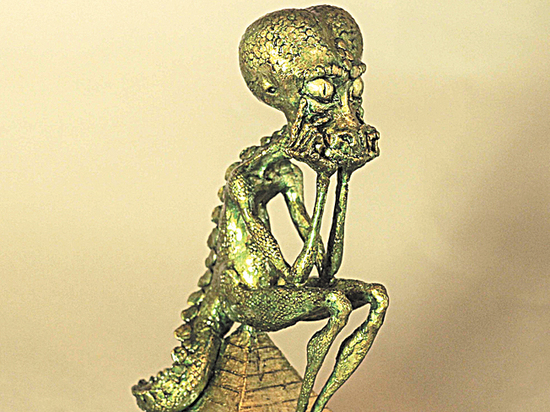
\includegraphics[width=10cm]{alyosha.png}
    \end{center}


    \item  $[+$15 в карму] Австралопитек Люси и гуманоид Алёшенька назначают другу другу свидание на планете Земля. Люси и Алёшенька прилетают независимо друг от друга на Землю в случайный момент времени, распределённый равномерно от 3 миллионов лет до падения Челябинского ме\-тео\-ри\-та и до 1 млн лет после него. Алёшенька ожидает Люси на Земле полмиллиона лет, а Люси ждет Алёшеньку один миллион лет. 
    
    Какова вероятность того, что они встретятся на планете Земля?
    
    % (16 - 3^2 / 2 - 3.5^2 / 2)/16 ~ 0.34
    
    Верное решение этой задачи вернет любимого научного руководителя.
    
    \item  $[+$15 в карму] 
    Яснопишущая в третьем поколении Глафира публикуется в журналах 
    минус первого квартиля. 
    Параметр интенсивности яснописания имеет равномерное распределение от 200 до 400 работ в год. 
    При заданной интенсивности яснописания количество опубликованных статей в год имеет распределение Пуассона. 
    
    \begin{enumerate}
        \item $[+$5 в карму] Найдите ожидаемое количество опубликованных за год статей.
        \item $[+$10 в карму] Найдите вероятность полного отсутствия публикаций у яснопишущей Глафиры за год.
    \end{enumerate}
    
    % a) E(X) = E(E(X|I)) = E(I) = 300
    % б) P(X=0) = E(exp(-I)) = 
    
    Верное решение этой задачи приворожит рецензента вашего диплома. 
    \newpage
    \item  $[+$15 в карму] 
    Согласно древнему пророчеству Ёкарного Бабая конец света
    должен наступить в случайный равномерный момент времени от 23:50 до полуночи.
    
    Если предсказание Ёкарного Бабая не сбывается до 23:59, 
    то электрик Петрович пытается устроить сбычу
    прогноза своими пассатижами ровно в полночь. 

    
    Электрик Петрович пьет кротовуху [Роспотребнадзор не рекомендует употреблять кротовуху на территории РФ] и, поэтому, может потерять пассатижи до полуночи с вероятностью $1/2$. Если Петрович теряет пассатижи, то устроить сбычу прогноза он не может. 
    
    Какова вероятность того, что сбычу прогноза устроил Петрович,
    если конец света наступил?

    % 0 (!) заметим, что конец света согласно пророчеству точно наступит до полуночи! 
    % а значит, действия Петровича в полночь значения уже не имеют
    
    Верное решение этой задачи открывает синюю чакру трезвости.     

    \item  $[+$15 в карму] 
    
    Число изгнанных демонов из Глафиры Петровны на лекции по волновому экзорцизму имеет 
    биномиальное распределение с ожидаемым количеством $80$ и дисперсией $16$. 
    
    Если хотя бы один демон изгнан, то лекция считается успешной. 
    
    Найдите корреляцию числа изгнанных демонов и индикатора успешности лекции. 
    
    Верное решение этой задачи зачисляет автоматом на курс демонической оптимизации. 
    
    % E(X) = 80, Var(X) = 16, p_x = 0.8, n = 100, 
    % E(Y) = 1- (1 - p_x)^100
    % E(XY) = 80
    % Var(Y) = (1- (1 - p_x)^100)(1 - p_x)^100 
    
\end{enumerate}

\newpage

Ответ на эту задачу 6/13, восстановите задачу.

\vspace*{1cm}

\begin{huge}
% \setlength{\baselineskip}{44pt}
В третье полнолуние декабря магисса в третьем поколении Агафья проводит обряд деления на ноль совместной 
вероятности для вызова духа сэра и сыра Томаса Байеса. Агафья успешно делит на ноль с вероятностью 0.5.
Если на ноль поделить удалось, то с вероятностью 0.6 появляется сэр Томас Байес. 
Если на ноль поделить не удалось, то с вероятностью 0.7 появляется сыр сэра Томаса Байеса. 

Найдите вероятность того, что поделить на ноль удалось, если появился не то сыр, не то сэр. 



\end{huge}
\vspace*{2cm}

    В редакцию «Прикладной ворожбы» пришло письмо. 

\vspace*{1cm}
 
    Меня зовут Наталья. Я преданная читательница вашего журнала уже 20 лет. 
    Расскажу немного о себе. Каждый день я варю борщ. Время приготовления борща имеет экспоненциальное распределение. До замужества я тратила на один борщ в среднем 30 минут.
    У меня в натальной карте 5 указаний на развод. 
    Каждое указание на развод повышает ожидаемое время приготовления борща на $10$ минут. 
    Я живу 10 лет с мужем и у нас все хорошо. Мы разведемся?

\vspace*{1cm}

    Помогите редакции ответить на письмо Натальи. 


\begin{comment}
сквозная нумерация задач!

Два раунда:

~90-120 минут решение задач

~90 минут Перудо

Роли:

закупка еды [Илья, Маша]

заряженная вода, аскорбинки анаферон

пиптца (~ 6 штук)

черные мусорные пакеты (50 штук)

одноразовая посуда 

салфетка

закупка кубиков [Алёна]

фотосъемка [Полина]

плейлист [Полина]
мистическая музыка, деревня дураков

распечатать задачи [Б]

распечатать правила Перудо (вики ок) [Б]

закупить книги в мцнмо [Б]

баннер с кашпировским на дверь

карты таро


\newpage

Каждая сложная задача +10 (15?) в карму

Каждая легкая задача дает +5 в карму

Допбаллы для тех, кто придет в шапочке из фольги

проверяем решения простых и сложных задач, ставим частичные баллы

Персонажи, теории и т.д.

Персонажи: Кашпировский, Чумак, Петрик, Фоменко, Эпштейн, Глоба, Джуна
гадалка Глафира Лукитична 
плоскоземельщик Лаврентий
ясновидящая Виола 
гадалка Фая 
маг Альмира 
регрессолог Константин
ворожея 
ведунья 
лжесоюз магов ШВЭ
бабушка всепомощница Зинаида 
парапсихолог 
экстрасенс 
таролог 
пишу прогнозы, моделирую события, снимаю всякого рода негативы, помогаю бороться с гомоскедастичностью 
приворот (бизнес и финансы) 
перекладываю эндогенность в регрессию рецензента 
Изольда работает по красной магии семи цветов 
При составлении натальной карты онлайн, определяется ваша космограмма на которую наносятся положения планет в домах и знаках зодиака на время вашего рождения. Далее по этим данным делается расшифровка гороскопа. 





выравнивание баллов: у вас не хватает заряда на долгое хранение огурцов.
Подбрасываем монетку с орлами с обеих сторон

указатели 



Теории, практики и их последователи: плоскоземельщики, гомеопаты (тут есть байка про кусочки Гитлера), свидетели НЛО/зеленых человечков, Новая хронология, 5G, чипы в вакцине, рептилоиды (Цукерберг!), гороскопы (совместимость козерогов со стрельцами) и прочая астрология и оккультизм, сонники, народная медицина/приметы, ауры, гадалки, экстрасенсы
Есть еще всякие менее известные/исторические штуки типа Пилтдаунского человека или гравицапы. Божествование Васильевой
Ещё в тему: https://nplus1.ru/news/2016/04/26/astral-go-go 



\newpage


Наброски задач

Кашпировский, Фоменко и еще кто-нть пошли в лес по грибы (за мухоморами, конечно) и подверглись нападению лис — любителей науки. Кашпировского (у меня  с ним личные счеты) покусали с вероятностью $р_1$, при этом он терял треть из собранных мухоморов, Фоменко -- с вероятностью $р_2$, и он терял половину ... тра-та-та

ОПГ из n лис пробрались в подвал к Чумаку и стали бить банки. Каждая лиса может разбить $\lambda_1$ банок в минуту. На шум прибежал Чумак и стал кидаться в лис мухоморами, попадая с вероятностью р. После первого попадания эффективность лисы падает до $\lambda_2$ банок в минуту. После второго попадания лиса уползает через вентиляцию и больше участия в оргии не принимает. Найдите матожидание числа разбитых банок (и, мб, оптимальную стратегию для Чумака - кидаться в свежих или уже подбитых)


Сообщения о высадке инопланетян поступают с частотой $\lambda_1$, в високосные годы — $\lambda_2$, а в годы, когда происходили полные солнечные затмения — $\lambda_3$. Посчитайте, сколько инопланетян должны были высадиться на Землю с полета Гагарина до конца света по календарю Майя

Описывая впечатления от назначения на должность, Васильева сказала, что ощутила "божествование". Вероятность, что журналист принял долженствование за божествование, равна тому-то, обратное – тому-то. В интервью оказалось божествование. Найдите вероятность того, что оно и было произнесено (что-то такое на Байеса) 

В городе N живет 30к человек. Для каждого из них вероятность вступить в секту плоскоземельщиков равна $р_1$, в ряды любителей анаферона – $р_2$, в число боящихся 5G – $р_3$. В период ретроградного Меркурия каждая из вероятностей увеличивается на …п.п. Какая доля населения будет состоять в нескольких сектах сразу?

Что-то про паранормальное распределение, функцию плотности ауры, закон распределения торсионных полей

Гадалка предсказывает значение, которое в реальности распределено так-то. Но тервера она не знает, и использует генератор случайных чисел с равномерным распределением. Какая выборка нужна, чтобы с такой-то уверенностью сказать, что предсказания – лажа? (Проверки гипотез у второго курса не было, но мб можно как-то переделать под предельные теоремы?)

Что-нибудь про пайплайн – очищение по Петрику + зарядка по Чумаку

На время закрытия станций зеленой ветки Мостранс рекомендует пользоваться «другими ветками метро, автобусами КМ, иноземным транспортом». Вы стоите на остановке и сядете в то, что первым придет. Прибытие автобусов КМ распределено по такому-то закону, а иноземного транспорта – по такому-то. На чем вы уедете с большей вероятностью/какова вероятность, что первым придет КМ?





\end{comment}


\end{document}